\textbf{Question 1}: Give a discussion of the parameter sensitivity of the Neural Transmitter Model, by multiplying \textbf{Alfa} ($\alpha$), \textbf{Beta} ($\beta$), \textbf{Gama} ($\gamma$) and \textbf{I0} ($I_0$) with 10, 5, 2, 1, 0.5, 0.2 and 0.1, respectively. The default values are: Alfa=2; Beta=5; Gama=0.5; and I0=1. Then comment on the role of each parameter.

For a biological neuron network, let's define:
\begin{table}[h]
    \centering
\begin{tabular}{c|c}
        \toprule
        \hline
\textbf{Item} & \textbf{Meaning}\\ \hline
I(t)          & Stimulus, \textbf{Input}\\
Z(t)          & Avaliable Neural Transmitters inside of the Synapse, \textbf{Response}\\
C(t)          &   Avaliable Neural Transmitters outside of the Synapse\\
              & where  \ce{I(t) + Z(t) <=>[$\gamma$ (come out)][$\alpha$ (come in)] C(t)}\\
$\alpha$      & Transmitter Depletion Rate (come in)\\
$\gamma$      & Transmitter Replenishment Rate (come out)\\
$\beta$       & $\beta$ = Z(t) + C(t) = Constant\\
S(t)          & Output Signal = I(t)Z(t), \textbf{Output}\\ \hline
\end{tabular}
    \caption{Def. of parameters}
    \label{tab:my_label}
\end{table}
\\
Then, the neuron transmitter dynamics equation can be written as:
\begin{equation}
    \dot Z = \alpha \left( {\beta  - Z} \right) - \gamma IZ
\end{equation}

(1) Play with the attached program in Matlab by multiplying parameters with 10, 5, 2, 1,
0.5, 0.2 and 0.1, plot out the responses in ONE figure for each parameter, e.g., with 7
different Alfa values and all other parameters in default values.
\\

\textbf{Solution 1-1}:
Please see the Figure \ref{fig:my_label1} to Figure \ref{fig:my_label4} for this question.

\begin{figure}
    \centering
    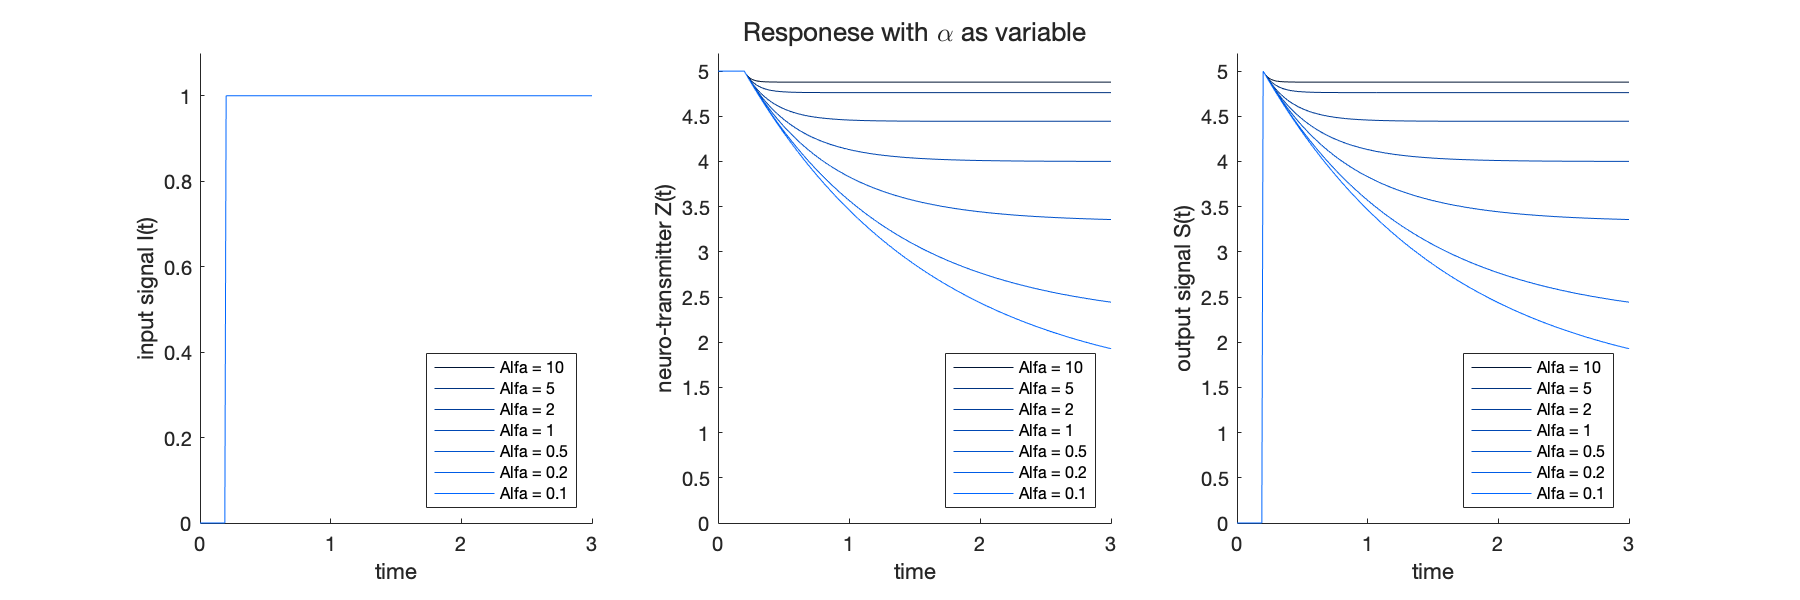
\includegraphics[scale=0.28]{picture/q1-1-1.png}
    \caption{Plot for Question-1 Step-1, where $\beta = 5, \gamma = 0.5, I_0 = 1$}
    \label{fig:my_label1}
\end{figure}
\begin{figure}
    \centering
    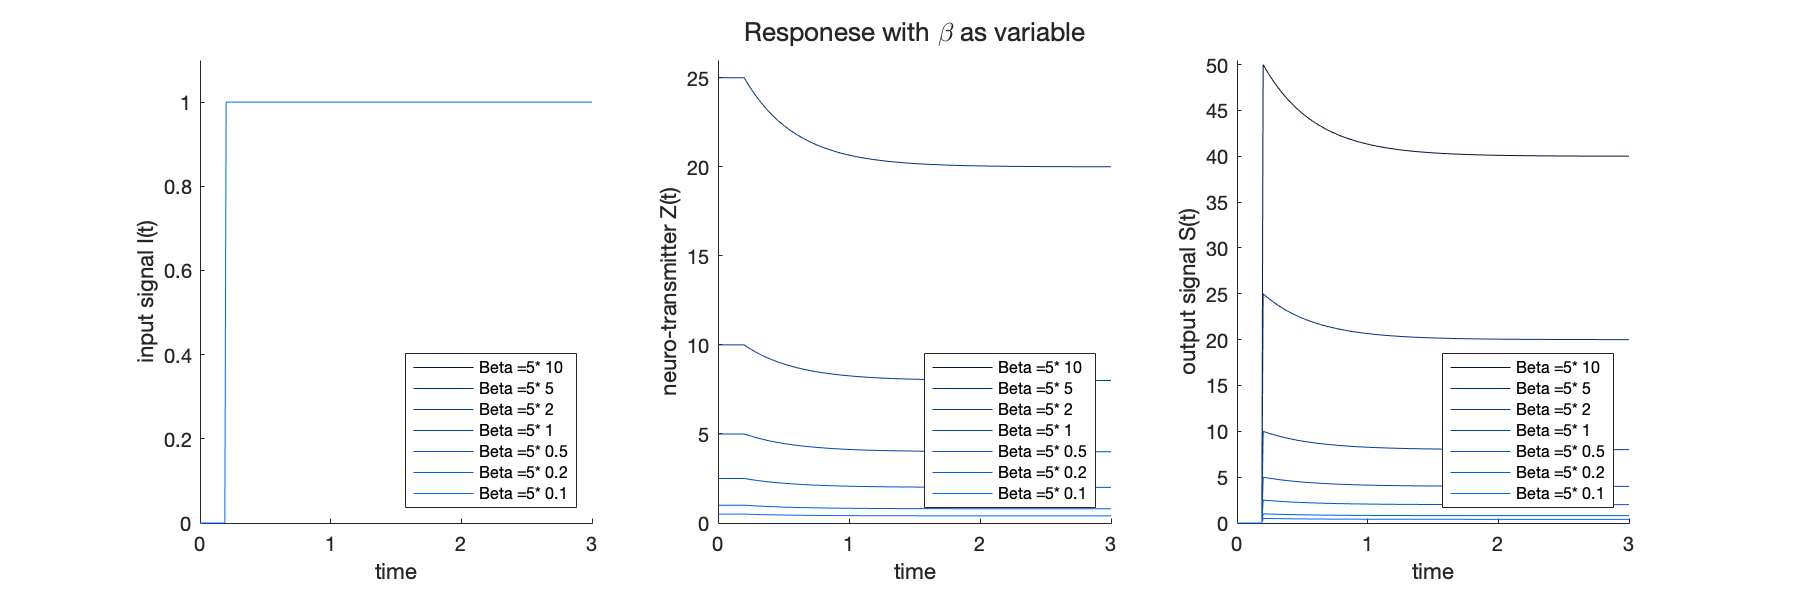
\includegraphics[scale=0.28]{picture/q1-1-2.png}
    \caption{Plot for Question-1 Step-1, where $\alpha = 2, \gamma = 0.5, I_0 = 1$}
    \label{fig:my_label2}
\end{figure}
\begin{figure}
    \centering
    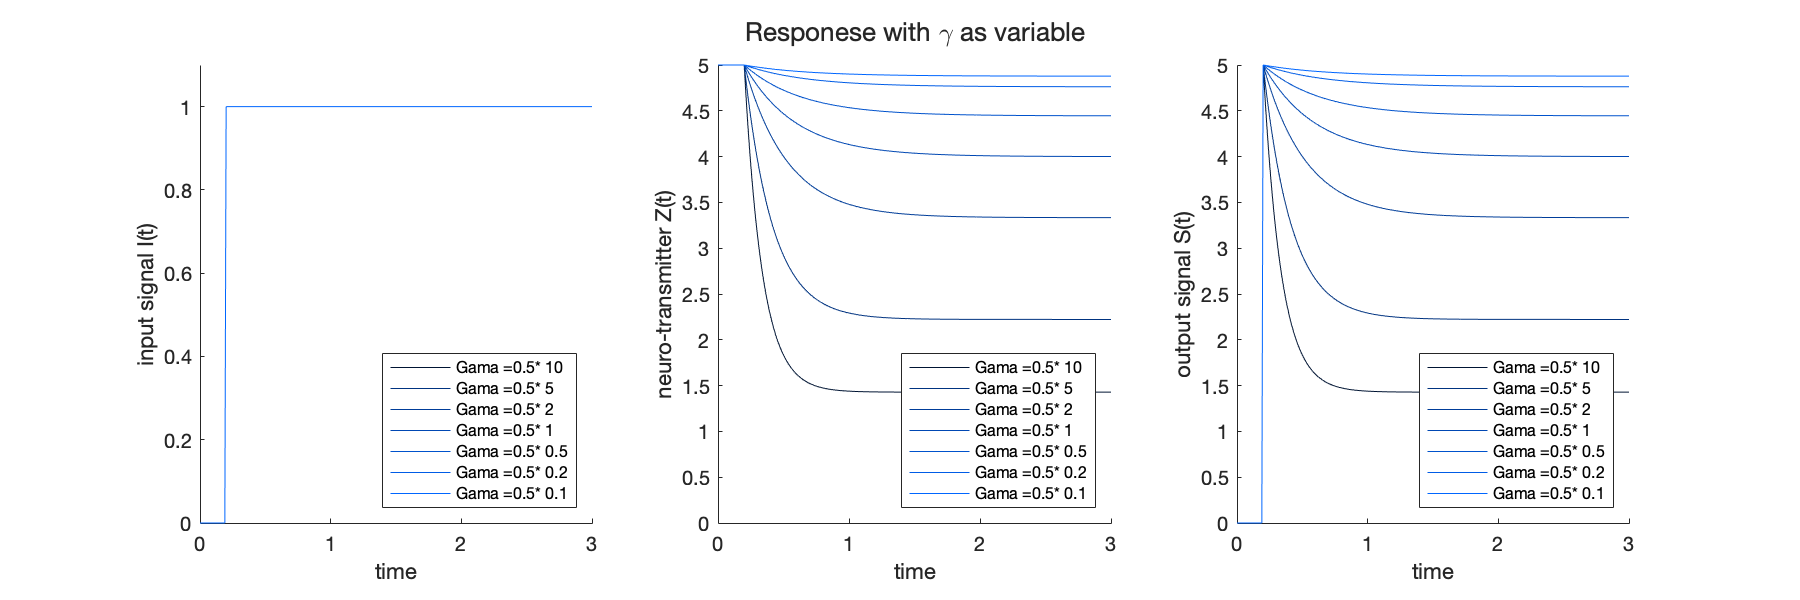
\includegraphics[scale=0.28]{picture/q1-1-3.png}
    \caption{Plot for Question-1 Step-1, where $\alpha = 2, \beta = 5, I_0 = 1$}
    \label{fig:my_label3}
\end{figure}
\begin{figure}
    \centering
    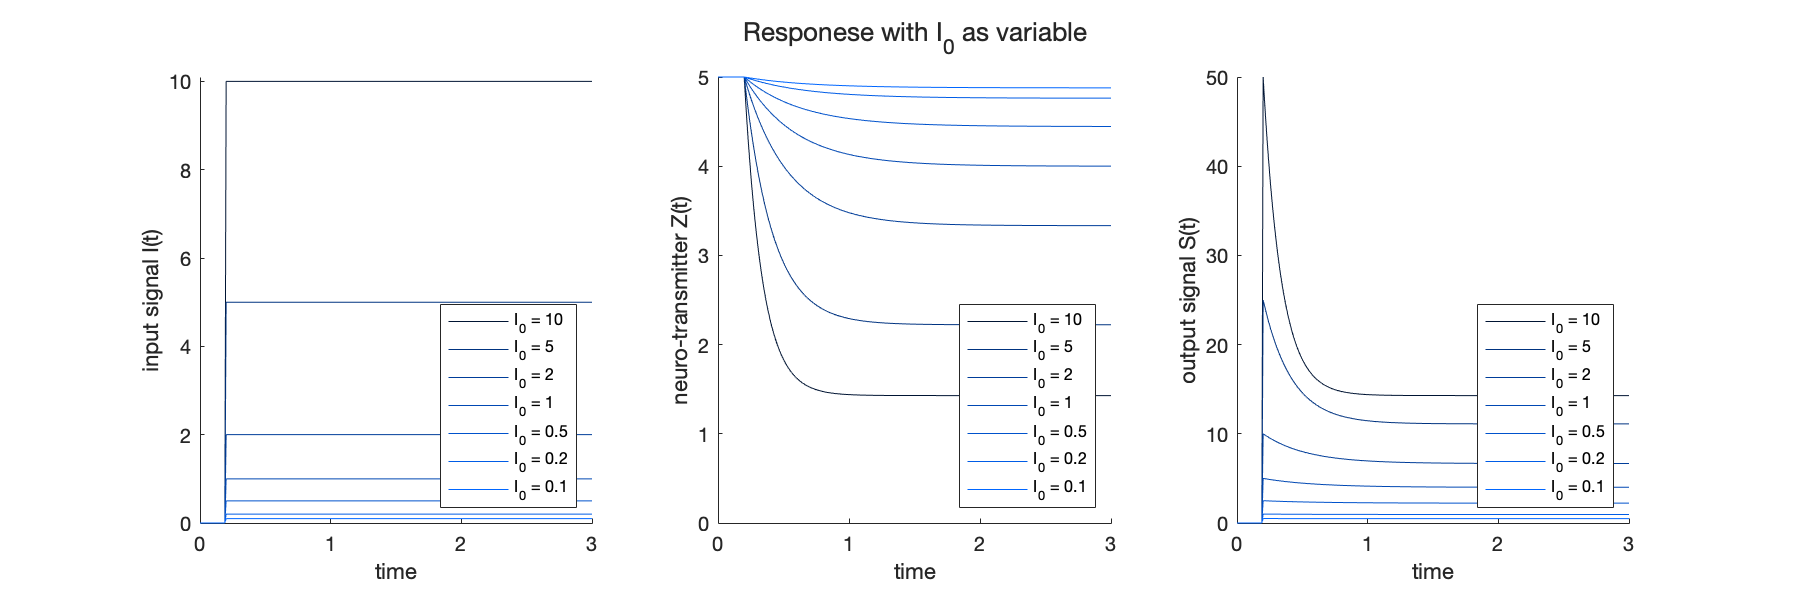
\includegraphics[scale=0.28]{picture/q1-1-4.png}
    \caption{Plot for Question-1 Step-1, where $\alpha = 2, \beta = 5, \gamma = 0.5$}
    \label{fig:my_label4}
\end{figure}


% \begin{figure}
%      \centering
%      \begin{subfigure}[b]{0.4\textwidth}
%          \centering
%          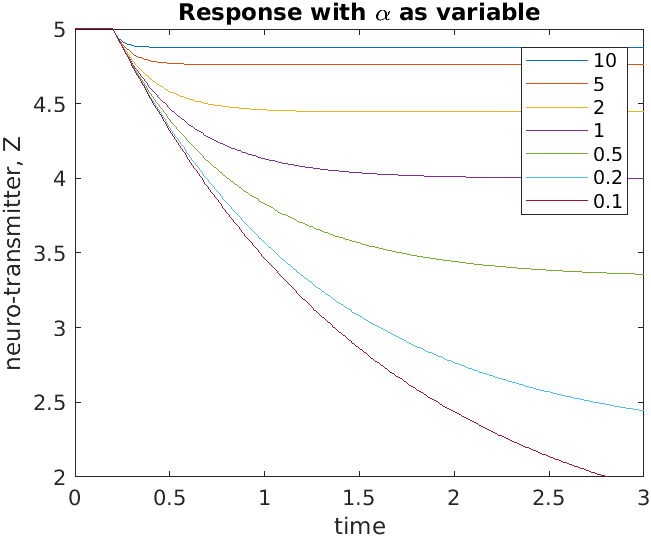
\includegraphics[width=\textwidth]{picture/Figure_alpha.png}
%          \caption{$\beta = 5, \gamma = 0.5, I_0 = 1$}
%          \label{fig:y equals x}
%      \end{subfigure}
%      \begin{subfigure}[b]{0.4\textwidth}
%          \centering
%          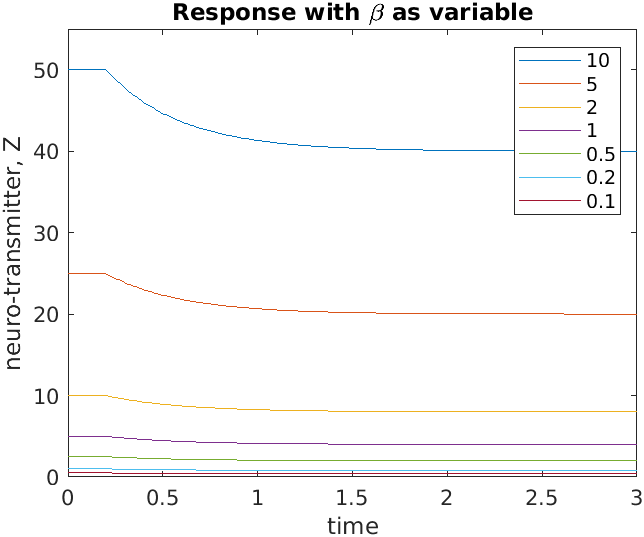
\includegraphics[width=\textwidth]{picture/Figure_beta.png}
%          \caption{$\alpha = 2, \gamma = 0.5, I_0 = 1$}
%          \label{fig:three sin x}
%      \end{subfigure}
%      \begin{subfigure}[b]{0.4\textwidth}
%          \centering
%          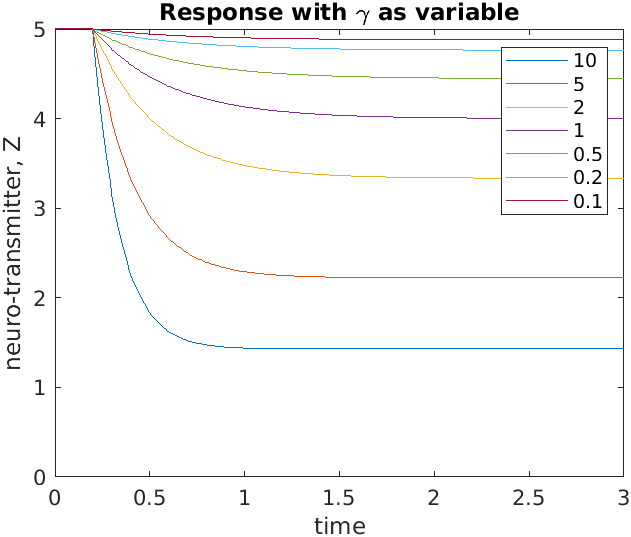
\includegraphics[width=\textwidth]{picture/Figure_gamma.png}
%          \caption{$\alpha = 2, \beta = 5, I_0 = 1$}
%          \label{fig:five over x}
%      \end{subfigure}
%     \begin{subfigure}[b]{0.4\textwidth}
%          \centering
%          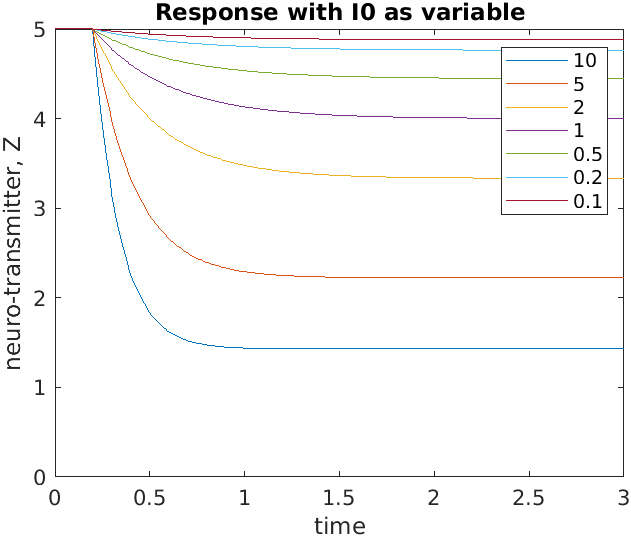
\includegraphics[width=\textwidth]{picture/Figure_I0.png}
%          \caption{$\alpha = 2, \beta = 5, \gamma = 0.5$}
%          \label{fig:five over x}
%      \end{subfigure}
%         \caption{The graphs for question 1-1}
%         \label{fig:fourgraphsforq1}
% \end{figure}


\\
(2) Similarly, find the relationship between the \textbf{overshoot} (calculate use the formula
given in class, do not measure it from figure) and parameters, respectively. Plot
figures of overshoot v.s. each parameter.

\\
\\
\\
\textbf{Solution 1-2}:
The equation for overshoot, A, is given by Equation \ref{eq1-2}:
\begin{equation}
    A = \beta {I_0} + \beta {I_0}\frac{\alpha }{{\alpha  + \gamma {I_0}}} = \frac{{\gamma \beta I_0^2}}{{\alpha  + \gamma {I_0}}} \label{eq1-2}
\end{equation}

We can easily see that the overshoot has a linear relationship with $\beta$ and $1/\alpha$, while has a non-linear relationship with  $\gamma$ and  $I_0$:

\[\begin{array}{l}
A \propto {\raise0.7ex\hbox{$1$} \!\mathord{\left/
 {\vphantom {1 \alpha }}\right.\kern-\nulldelimiterspace}
\!\lower0.7ex\hbox{$\alpha $}}\\
A \propto \beta \\
A \propto \frac{C_1}{\frac{1}{\gamma}+C_2} \\
A \propto \frac{1}{{\left( {\frac{{{C_3}}}{{I_0^2}}} \right) + \left( {\frac{{{C_4}}}{{{I_0}}}} \right)}}
\end{array}\]
\\
\begin{figure}[h]
     \centering
     \begin{subfigure}[b]{0.4\textwidth}
         \centering
         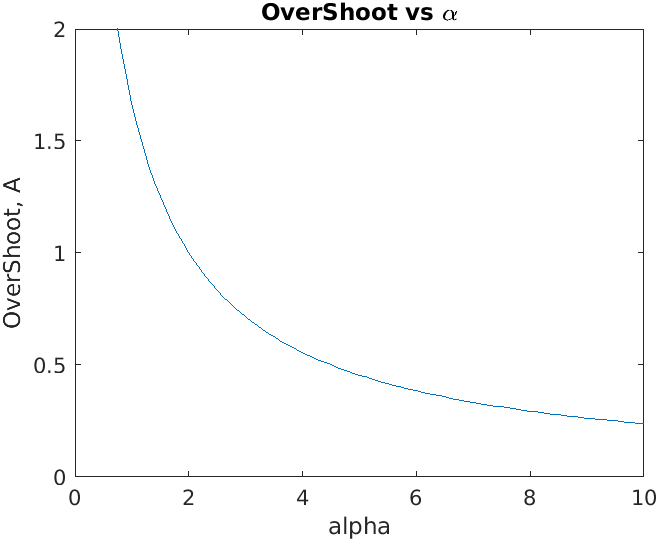
\includegraphics[width=\textwidth]{picture/Figure_1-2alpha.png}
         \caption{$\beta = 5, \gamma = 0.5, I_0 = 1$}
         \label{fig:y equals x}
     \end{subfigure}
     \begin{subfigure}[b]{0.4\textwidth}
         \centering
         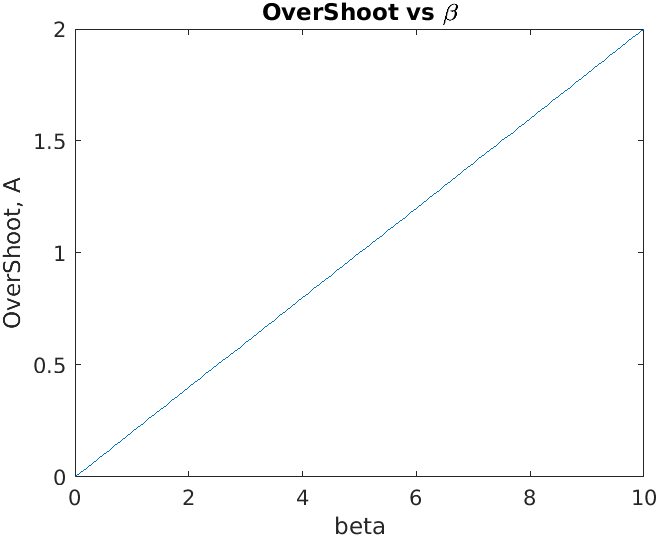
\includegraphics[width=\textwidth]{picture/Figure_1-2beta.png}
         \caption{$\alpha = 2, \gamma = 0.5, I_0 = 1$}
         \label{fig:three sin x}
     \end{subfigure}
     \begin{subfigure}[b]{0.4\textwidth}
         \centering
         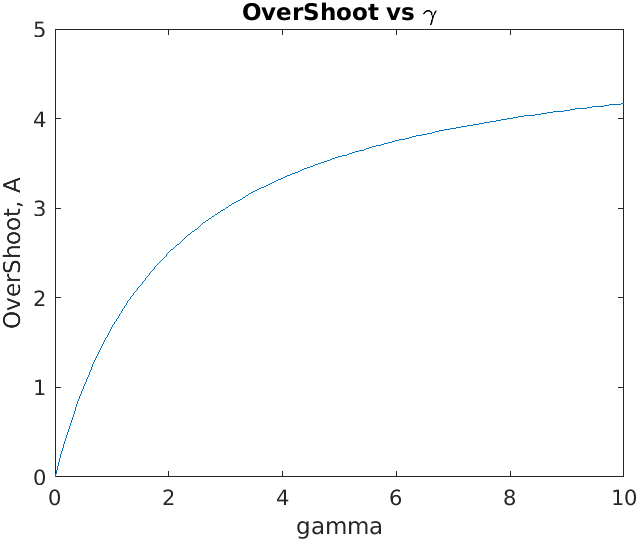
\includegraphics[width=\textwidth]{picture/Figure_1-2gama.png}
         \caption{$\alpha = 2, \beta = 5, I_0 = 1$}
         \label{fig:five over x}
     \end{subfigure}
    \begin{subfigure}[b]{0.4\textwidth}
         \centering
         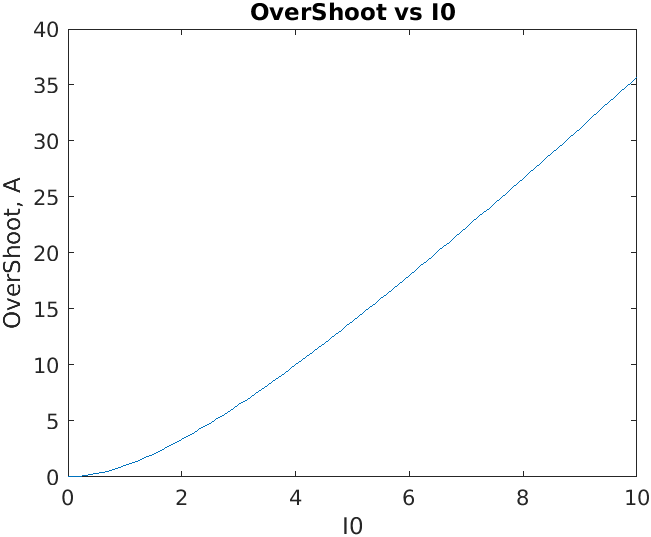
\includegraphics[width=\textwidth]{picture/Figure_1-2I0.png}
         \caption{$\alpha = 2, \beta = 5, \gamma = 0.5$}
         \label{fig:five over x}
     \end{subfigure}
        \caption{The graphs for Question-1 Step-2}
        \label{fig:fourgraphsforq2}
\end{figure}
\\
Please refer to Figure \ref{fig:fourgraphsforq2} for each of the plots for this question.
\\
(3) Similarly, find the relationship between the time constant and parameters, respectively. Plot figures of time constant v.s. each parameter.

\textbf{Solution 1-3}: The equation of $\tau$ is given in Equation \ref{eq1s3}:
\begin{equation}
    \tau = \frac{1}{\alpha+\gamma I}\label{eq1s3}
\end{equation}

\\
\begin{figure}[h]
     \centering
     \begin{subfigure}[b]{0.3\textwidth}
         \centering
         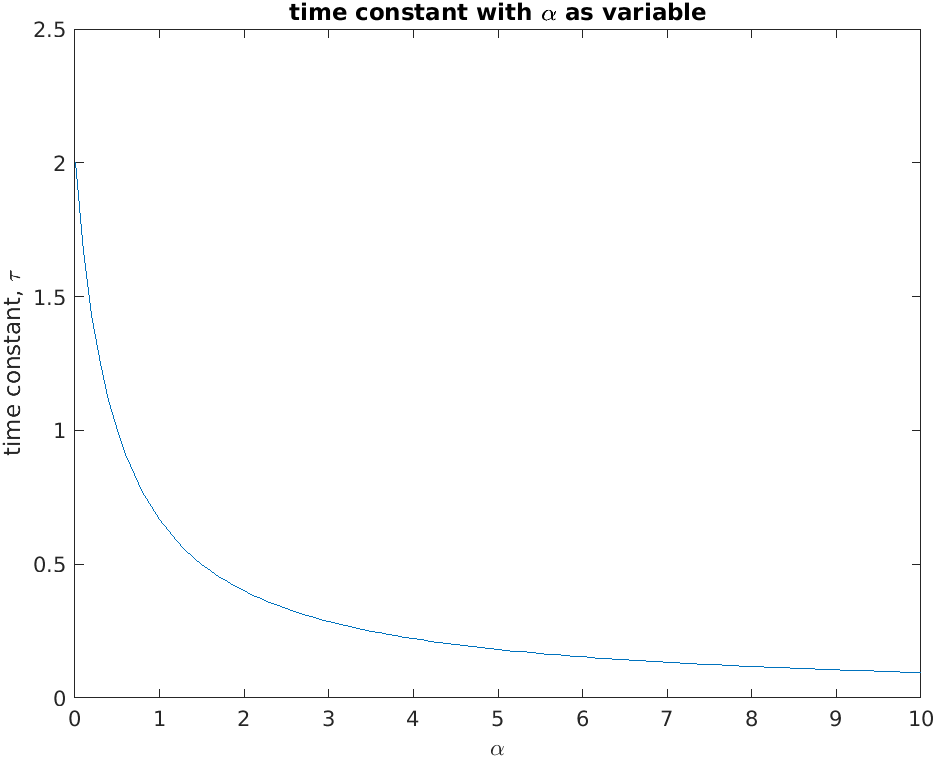
\includegraphics[width=\textwidth]{picture/Figure_1-3alpha.png}
         \caption{\gamma = 0.5, I_0 = 1$}
         \label{fig:y equals x}
     \end{subfigure}
     \begin{subfigure}[b]{0.3\textwidth}
         \centering
         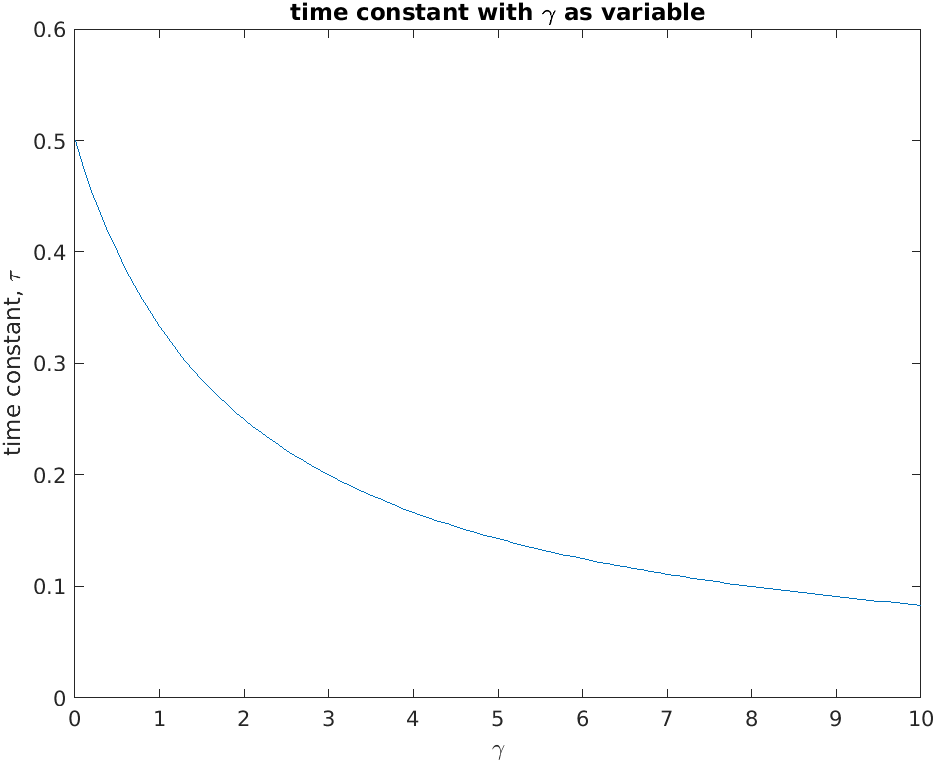
\includegraphics[width=\textwidth]{picture/Figure_1-3gamma.png}
         \caption{$\alpha = 2, I_0 = 1$}
         \label{fig:three sin x}
     \end{subfigure}
     \begin{subfigure}[b]{0.3\textwidth}
         \centering
         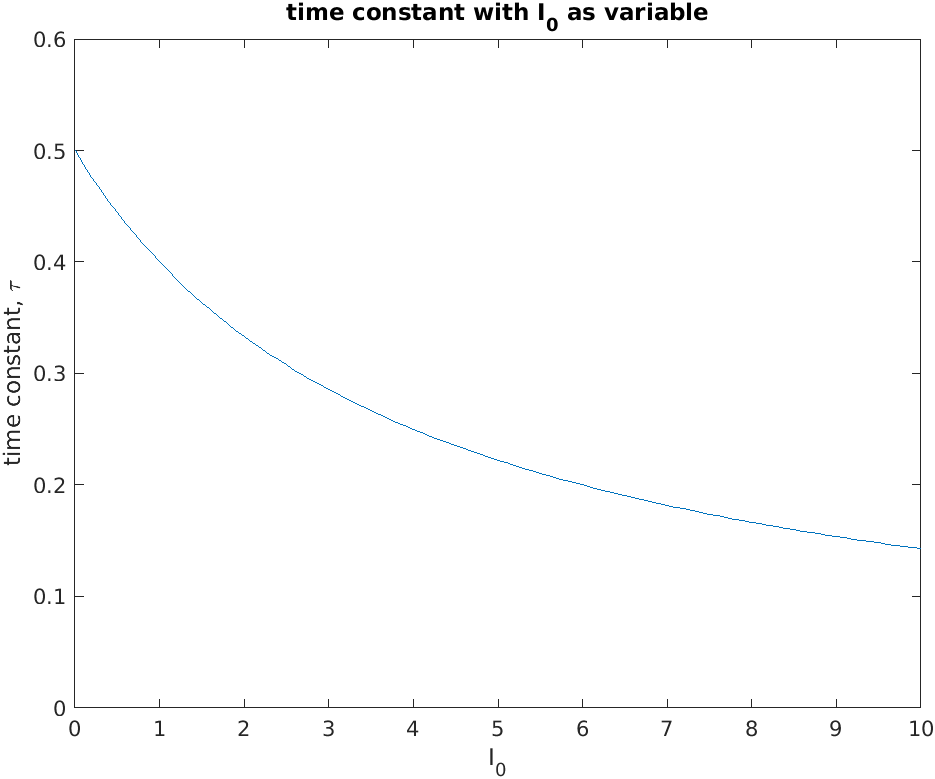
\includegraphics[width=\textwidth]{picture/Figure_1-3I0.png}
         \caption{$\alpha = 2, \gamma = 0.5$}
         \label{fig:five over x}
     \end{subfigure}
        \caption{The graphs for Question-1 Step-3}
        \label{fig:fourgraphsforq3}
\end{figure}
Please see Figure \ref{fig:fourgraphsforq3} for the plots of this question.


\textbf{Give a discussion of the parameter sensitivity, and comments on each parameter:}
\\As per June-10's lecture note, parameter sensitivity is defined as the slop on the output signal vs. parameter plot. 

The $\alpha$ and $\gamma$ are the come in/out rate, $\Delta S$ is sensitive to  $\alpha$ and $\gamma$ at steady state. $\Delta S$ has an nonlinear relationship with $\alpha$ and $\gamma$ , as we can see from the plots above, the magnitude of $\Delta S$ decrease with $\alpha$ and increase with $\gamma$, so they are important parameters to $S$. 

The $\beta$ and $I_0$ are the total number of transmitters and input signal.  $\Delta S$ is not a function of $\beta$ , so $\beta$ is not important parameter; while, $I_0$ has a non-linear impact on the $\Delta S$, which is very similar as $\gamma$, so we conclude that $I_0$ is an important parameter.

\\
\clearpage
\pagebreak
\textbf{Question 2}: Give a discussion of the parameter sensitivity of the \textbf{Shunting Model}, by multiplying\textbf{ A, B, D} with 10, 5, 2, 1, 0.5, 0.2 and 0.1, respectively. The positive and negative inputs are:
\[S+ = I_{ex} \cdot u(t-t_{ex})\]
\[S- = I_{in} \cdot u(t-t_{in})\]

respectively, where constants $I_{ex} = I_{in} = 1$ are the amplitude of the inputs. Constants $t_{ex} = 0.2$ and $t_{in} = 0.8$ are the on-set time of the positive and negative inputs, respectively.
Function $u(t-t_0)$ is the unit step function defined as:
\[u(t- t_0) = 1, \quad \mathrm{if \quad} t>0\]
\[u(t- t_0) = 0, \quad \mathrm{otherwise}\] The \textit{default} values are: A=10; B=1; D=1. 
Then comment on the role of each parameter.
\\
\textbf{Steps}:
\\
(1) This question is similar to Question 1, except it has two inputs. By slightly modifying the program in the Appendix 1, you will get the results. The response of the shunting model with default parameter values is in Appendix 2.

\\
(2) In the Matlab program with default parameter value, the maximum time is set as 150*0.01=1.5. However, in some case, you may need a longer time to see the response to reach its steady state.


\begin{figure}[h!]
    \centering
    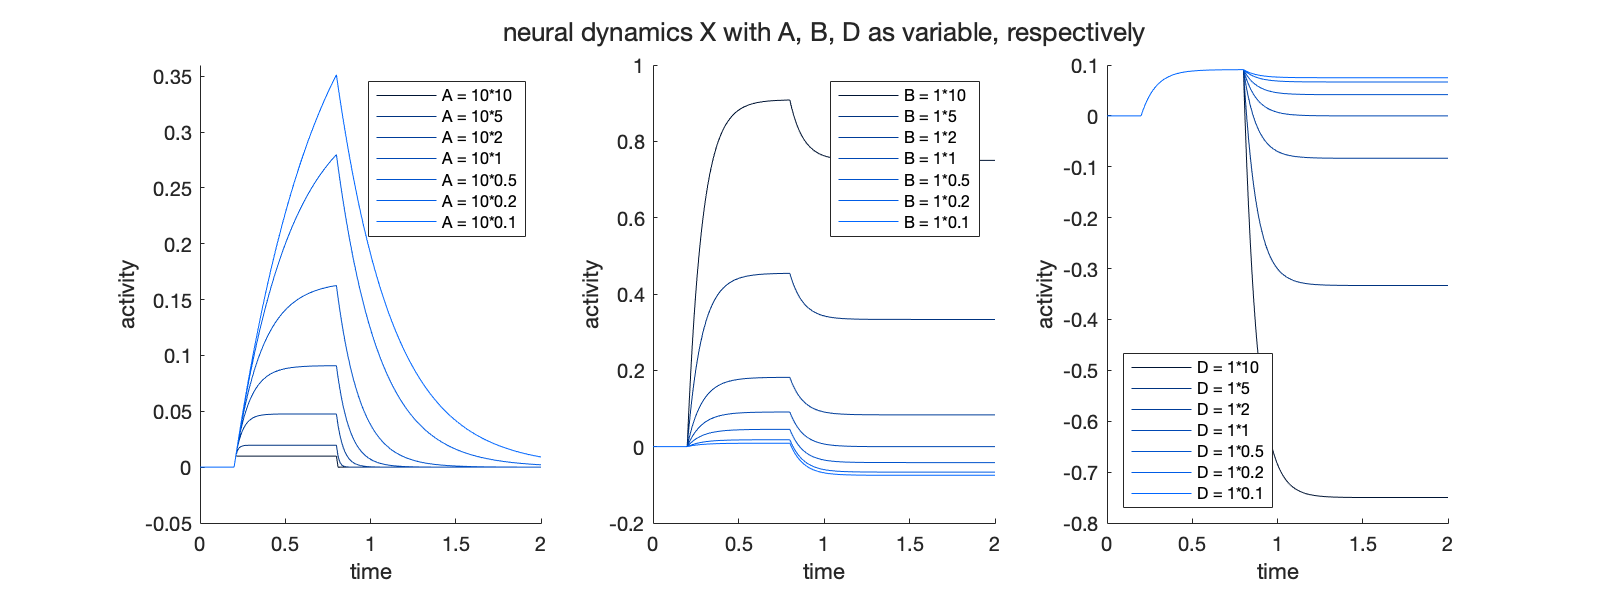
\includegraphics[scale=0.30]{picture/q2-1.png}
    \caption{Plot for Question-2 Step-1 and 2}
    \label{fig:my_label7}
\end{figure}

\\
\\

\textbf{Give a discussion of the parameter sensitivity, and comments on each parameter:}

\\As per June-10's lecture note, parameter sensitivity is defined as the slop on the output signal (Activity, X) vs. parameter plot.

\\$A$ is the positive decay, while, $B$ and $D$ are the upper and lower bounds.

\\As we can see from the plots above, $\Delta X$ is a non-linear function of A, while, not a function of $B$ and $D$ (The shape and slope of the plot does not change with $B$ and $D$), so we save A is an important factor; while, B and D are not important factors. So $X$ is sensitive to $A$ 

